% Chapter Template

\chapter{Introduction} % Main chapter title

\label{Introduction} % Change X to a consecutive number; for referencing this chapter elsewhere, use \ref{ChapterX}

%----------------------------------------------------------------------------------------
%	SECTION 1
%----------------------------------------------------------------------------------------
\section{Data Joins}
\subsection{Background}
Over the recent years, technology has been growing rapidly. It is now easier to collect data. Combined with the large volume of data we already have in archives, there are many data sets we can use to perform statistical analysis on. The problem is that even though there are many data sets we can use, it is not common to have one set of data which contains everything we want. One example is regional data. If we wish to do statistical analysis on the all regions, we would need combine multiple data sets together. Most analysis functions in common statistical analysis software only take in one data set.

To solve this problem we can merge the data sets together, in a process that is also known as "data joins". There are many ways we can join these data sets together but it seems like there are not much tutorials that explicate the manipulation of data structures.
Therefore, we should focus on how to educate this in an descriptive manner, with this being said we will create a set of animations for a few common data joins. 

\subsection{Current approach of teaching data joins}
\subsubsection{Text Approach}
Understanding how these joining operations work and how to use them can be challenging. Some people can do it by imagining the data structure but those who can’t would have a difficult time to learn them just from reading about them.

One explanation found about left joins is that it "returns all rows from the left table, even if there are no matches in the right table". For those who are familiar with joins, this may seem obvious and easy to understand but for those who are not may not understand what "no matches" mean. No matches actually means that there are no identical key columns. 

\subsubsection{Venn Diagrams (Static)}
When it comes to images, Venn diagrams are the most popular way of teaching \textsf{SQL} joins. If we try to search for “SQL join tutorials”, we will see Venn diagrams everywhere (See Fig.~\ref{fig:vennsearch}).

\begin{figure}[H]
    \centering
    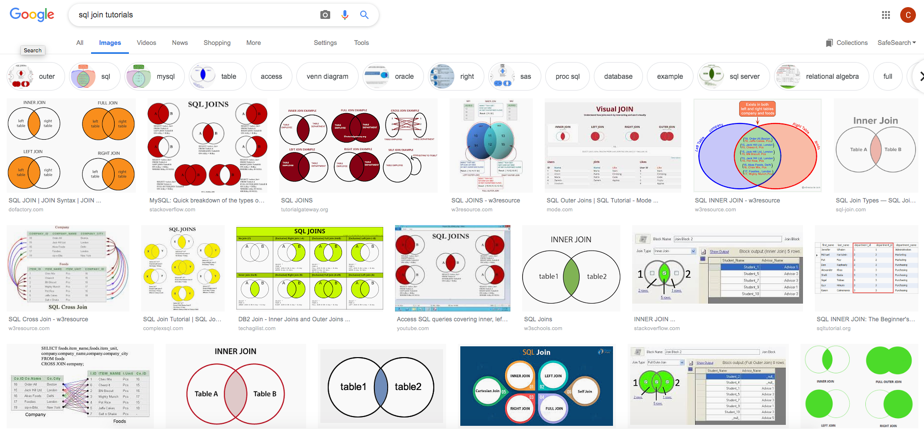
\includegraphics[scale = 1.0]{Masters-Thesis/img/vennsearch.png}
    \caption{\textsf{SQL} join tutorials}
    \label{fig:vennsearch}
\end{figure}

\begin{figure}[H]
    \centering
    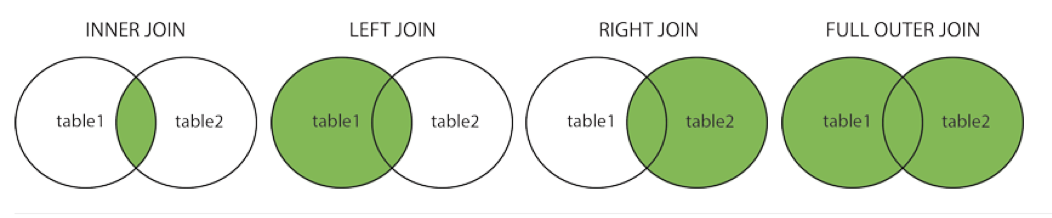
\includegraphics[scale = 0.8]{Masters-Thesis/img/venn.png}
    \caption{\textsf{SQL} Join Venn diagrams}
    \label{fig:venn}
\end{figure}

Although diagrams like Fig.~\ref{fig:venn} are a popular way of teaching joins, there are many problems with them.

\begin{itemize}
    \item Venn diagrams are useful in probability because we can think of the diagrams as sets and we can see visually what intersects or unions are. However, when it comes to data joins, the diagrams don’t look like data tables.
    \item They are too vague about how the joins work. For example "inner join" isn’t just the intersect of two tables, there is much more to it. 
    \item The multiple type of joins are similar in terms of how the rows from different tables are joined together. The essential differences are in how they treat missing values.
\end{itemize}

Regardless of the problems, the useful features are,

\begin{itemize}
    \item The structure of joins are shown. For example, the left join is information from table 1 plus the intersection of table 1 and table 2. Full join is the combination of table 1 and table 2. They are not incorrect, just insufficient. 
    \item These Venn diagrams show us which rows ends up represented in the join but do not tell us anything about how the rows are joined together.
    \item These diagrams would be a useful visual resource to explain the basic structure of the joins, they are just not suitable to be the only such resource. 
\end{itemize}


\newpage

\subsection{R for Data Science Approach}
In their influential book R for Data Science, \citet*{Wickham:2017:RDS:3086927} have a section explaining different type of joins. They did not use Venn diagrams to convey the idea of joins, however, they did use Venn diagrams for other purposes, so this omission is significant. 

\begin{figure}[H]
    \centering
    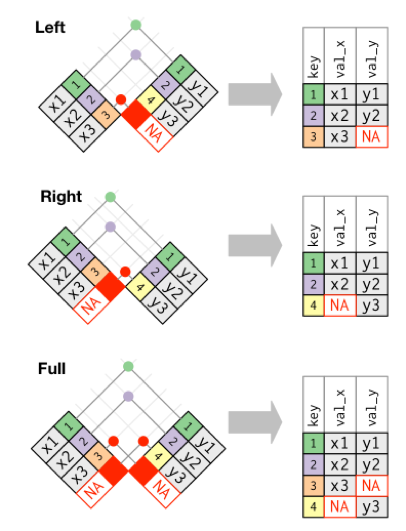
\includegraphics[scale = 1.0]{Masters-Thesis/img/r4djoin.png}
    \caption{Data Join Diagrams in R for Data Science}
    \label{fig:r4djoin}
\end{figure}


Instead, they show two separate tables as in Fig.~\ref{fig:r4djoin}, where each row is coloured differently. Then, there lines which link the rows together indicating that these rows are joined together. At the end there is a result table. \\

The advantages of this approach compared to Venn diagrams.
\begin{itemize}
    \item Each table and rows in all tables are shown nicely.
    \item There are line linking rows that are matched together, and also unmatched rows.
    \item There is a result table showing what the table would look like after being joined.
\end{itemize}
	
What is missing from this approach.

\begin{itemize}
    \item For those who are not familiar with these joins, it would be difficult for them to understand it without any verbal descriptions.
    \item They are very cryptic and they do not show effects of multiple matches.
    \item Matching rows are shown by having the same colour when there more rows, eventually unique colours will run out.
    \item There are no messages showing why the linked rows are joined together or why some rows disappears after being joined.
\end{itemize}

With the technology we have today, the ultimate goal would be to use animations to convey the idea of joins. 

\subsubsection{Dynamic Approach}

Static images have been used as the main approach of teaching data joins for a long time, the limitation and lack of features has been explained in the previous sections. So, a new yet better approach should be used, a dynamic approach would be more appropriate.
There are many advantages of using animations for teaching purposes. The main one is that humans are more attracted to moving things. They can also focus on them for longer. “This behavioural pattern is rooted deeply in our animal instincts as well as our ancestors’ need for self-preservation. In order to keep us safe, our brains have a built-in mechanism that keeps us aware of everything happening around us” \footnote[1]{\href{https://blog.gallereplay.com/static-vs-dynamic-the-psychology-behind-cinemagraphs/}{https://blog.gallereplay.com/static-vs-dynamic-the-psychology-behind-cinemagraphs/}}. \\

Recently, a set of data joining animations called \href{https://github.com/gadenbuie/tidyexplain}{\textbf{tidyexplain}} \citep{tidyexplain} on \textsf{Github} (see Fig.~\ref{fig:tidyejoin}), were created with the \textbf{gganimate} \citep{gganimate} \textsf{R} package.

\begin{figure}[H]
    \begin{tabular}{cc}
     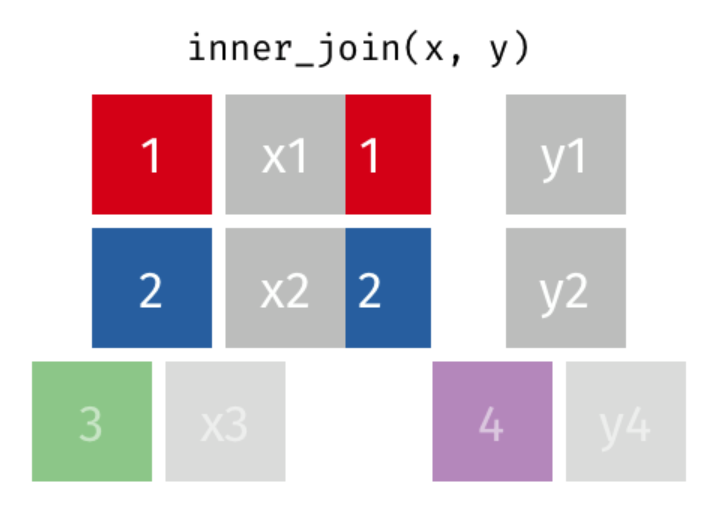
\includegraphics[scale = 0.25]{Masters-Thesis/img/gginnerj.png} & 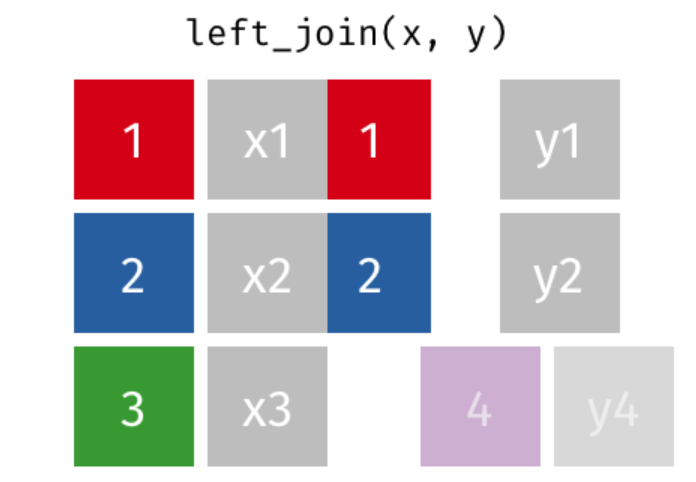
\includegraphics[scale = 0.25]{Masters-Thesis/img/ggleftj.png} \\
    (a) Inner Join & (b) Left Join \\[6pt]
     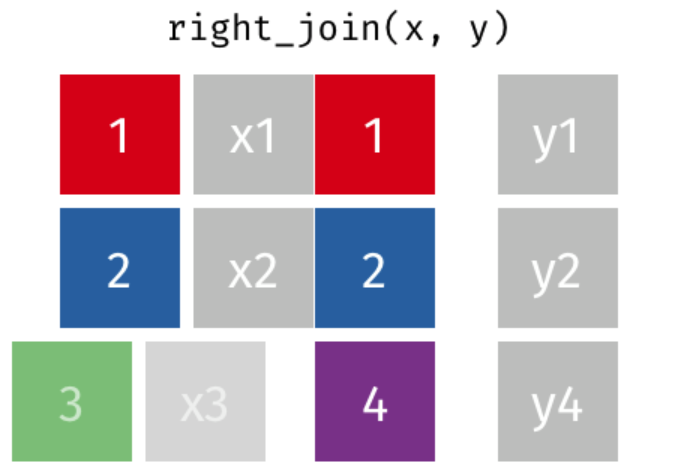
\includegraphics[scale = 0.25]{Masters-Thesis/img/ggrightj.png} & 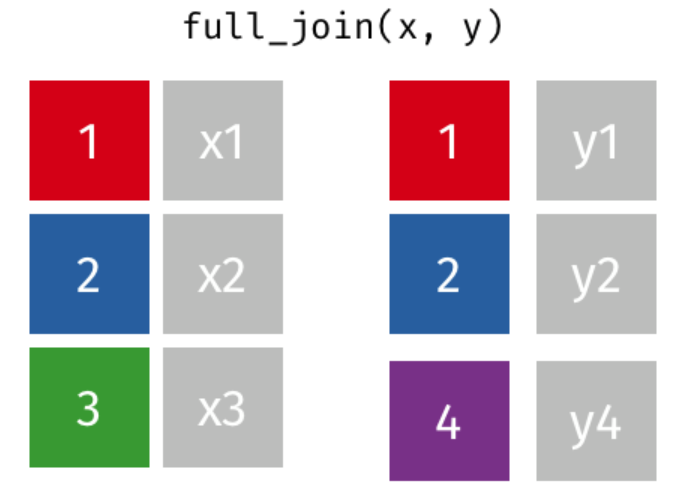
\includegraphics[scale = 0.25]{Masters-Thesis/img/ggfullj.png} \\
    (c) Right Join & (d) Full Join \\[6pt]
    \end{tabular}
    \caption{Joining animations in \textbf{tidyexplain}}
    \label{fig:tidyejoin}
\end{figure}

These animations are really similar to the images from the R for data science book, so most of the limitations still remains. The animation lack explanations of how unmatched rows are treated. Although the limitations remain, the advantage of these animations is that the users are given a better picture of how matched rows are joined together. 
\\
In the next section, we will talk about data reshaping which is also an important part of data pre-processing. 

\section{Data Reshaping}
\subsection{Background}
A popular quote \textit{"often 80\% to 90\% of a data analysis project is spent in making the data reliable enough that the results can be trusted"} \citep{Johnson2003DataQA}.  This is true, because often we do not receive the data set in the form we want, they are often messy and may take time to transform them into a desired tidy form. It can also be difficult to reshape the data set into the shape that we want.  Basically we can break the data pre-handling process into two parts, data cleaning and data tidying. We will focus on the latter one, since data tidying is an important aspect. Therefore, we should educate this with a visualisation where we can allow users to see the process of data reshaping. With this being said, we will create a set of animation for two aspects this.

\subsection{Tidy data}
The idea of the tidy data is that every row is an observation and every column is a variable as shown in Fig.~\ref{fig:hadtidyd}, this shape of data is used the most in statistical analysis software. \\

\begin{figure}[H]
    % \centering
    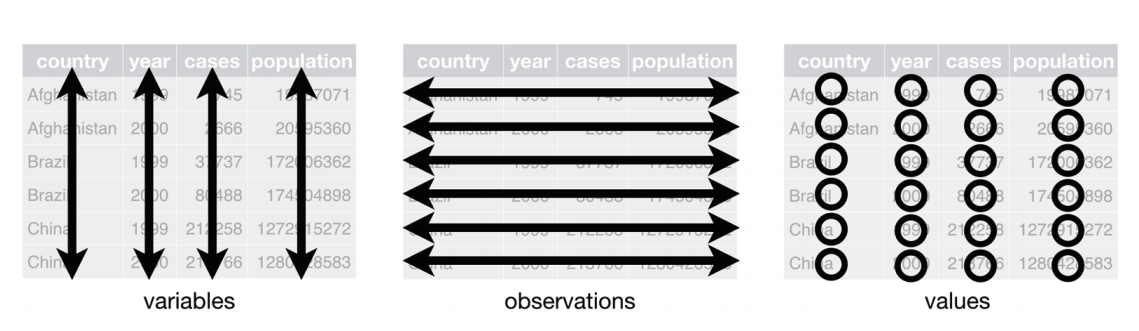
\includegraphics[scale = 0.35]{Masters-Thesis/img/hadtidyd.png}
    \caption{Tidy data \citep{Wickham:2017:RDS:3086927}}
    \label{fig:hadtidyd}
\end{figure}

However, different software or different functions within a software may take in data sets in various shapes. Below we have the same data set in two shapes, a wide one at Table~\ref{t:wided} and a long one at Table~\ref{t:longd}. \\

\begin{table}[H]
\centering
\begin{tabular}{rrrr}
  \hline
patient & sex & treatment\_num & value \\ 
  \hline
1 & M & treatment1 & 13.90 \\ 
2 & F & treatment1 & 90.40 \\ 
3 & F & treatment1 & 15.50 \\ 
4 & M & treatment1 & 12.70 \\ 
1 & M & treatment2 & 42.25 \\ 
2 & F & treatment2 & 16.13 \\ 
3 & F & treatment2 & 48.84 \\ 
4 & M & treatment2 & 19.36 \\ 
1 & M & treatment3 & 98.60 \\ 
2 & F & treatment3 & 48.04 \\ 
3 & F & treatment3 & 33.43 \\ 
4 & M & treatment3 & 4.86 \\ 
   \hline
\end{tabular}
\caption{Long data set}
\label{t:longd}
\end{table}

\begin{table}[H]
\centering
\begin{tabular}{rrrrr}
  \hline
patient & sex & treatment1 & treatment2 & treatment3 \\ 
  \hline
1 & M & 13.90 & 42.25 & 98.60 \\ 
2 & F & 90.40 & 16.13 & 48.04 \\ 
3 & F & 15.50 & 48.84 & 33.43 \\ 
4 & M & 12.70 & 19.36 & 4.86 \\ 
   \hline
\end{tabular}
\caption{Wide data set}
\label{t:wided}
\end{table}

For example, if we want to fit some common models like a regression, we would want the data to be in the wide form, because we want every variable to be in its own column. However, if we want to do a mixed model then we would want the data in a long form. Another advantage of the long data set is that it allows us to produce some plots which we can separate by groups like a box plot by treatment, because we will need a column as an indicator. Therefore, it is important for users to truly understand the underlying process of how reshaping from long to wide or wide to long work. In the next section we will discuss briefly how we can do this in \textsf{R}.

\subsection{Reshaping in \textsf{R}}
In \textsf{R}, to transform the data from wide to long, we can simply use the \texttt{gather()} function from the \textbf{tidyr} package.
\begin{lstlisting}
> data(toyda_wide)
> data_long = toyda_wide %>% gather(Subject, Score, 
    English, Maths)
> data_long
# Name Subject Score
# Alex English  92.2
#  Ben English  63.7
#  Sam English  75.6
# Alex   Maths  88.8
#  Ben   Maths  10.0
#  Sam   Maths  52.9
\end{lstlisting} \\

The \texttt{key} argument allows us to define the new column we wish create in the new table to store old columns from the original table. For example, we are trying to store columns English and Maths from the wide data into one column named Subject in the new table.

The \texttt{value} argument allows us to define the new column to store any values which are in the original data, these are the original values under columns English and Maths

The rest of the parameters are the columns we wish to transform on. \\

Similarly, for wide to long we can use the \texttt{spread()} function, we can think of this as an inverse of the long to wide transformation
\begin{lstlisting}
> data(toyda_long)
> data_wide = toyda_long %>% spread(Subject, Score)
> data_wide
# Name English Maths
# Alex    92.2  88.8
#  Ben    63.7  10.0
#  Sam    75.6  52.9
\end{lstlisting}

The \texttt{key} argument lets us define which column we wish to spread into multiple columns, here, we are trying to spread the Subject column into multiple columns English and Maths.

The \texttt{value} lets us define which column contains that corresponding values of the key column (we provided this in the previous argument). These values will then be transformed into the multiple columns that we created. 

\subsection{Current approach of teaching data reshaping}

\subsubsection{R for Data Science Approach}

Again, in the influential book R for Data Science there is a chapter explaining tidy data. Their approach is rather simple, they used a static image with dull grey scale colouring and arrows pointing where each elements from the old table should go into the new table.

\begin{figure}[H]
    \centering
    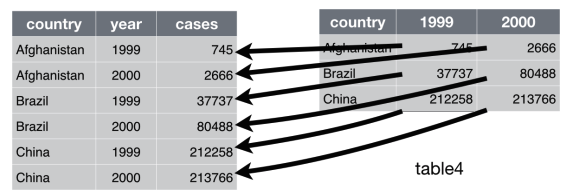
\includegraphics[scale = 0.5]{Masters-Thesis/img/r4dsw2l.png}
    \caption{Wide to Long, R for Data Science}
    \label{fig:r4dsw2l}
\end{figure}

\begin{figure}[H]
    \centering
    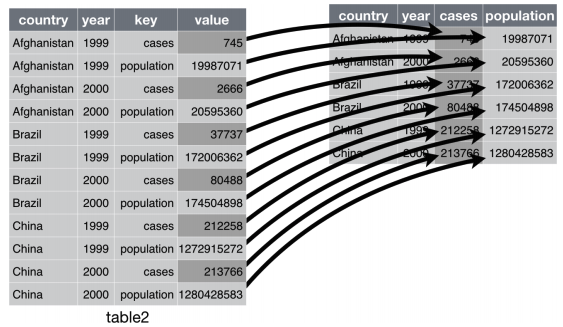
\includegraphics[scale = 0.5]{Masters-Thesis/img/r4dsl2w.png}
    \caption{Long to Wide, R for Data Science}
    \label{fig:r4dsl2w}
\end{figure}

There are not much advantages of this approach except for giving the user a basic idea of how the transformation works. \\

However, the limitations are.
\begin{itemize}
    \item Not obvious to the user what the images are trying to explain.
    \item Does not annotate how "1999" and "2000" are used. 
    \item Arrows overprinting on the table makes the table difficult to read.
    \item Lack of annotations of what the steps are.
\end{itemize}

\subsubsection{Dynamic Approach}


As explained before in the previous sections, a set of data joining animations called \href{https://github.com/gadenbuie/tidyexplain}{\textbf{tidyexplain}}  on \textsf{Github} (see Fig.~\ref{fig:tidyejoin}), were created with the \textbf{gganimate} \textsf{R} package. They also have another set of animations for data reshaping (See Fig.~\ref{fig:tidyel2w} and Fig.~\ref{fig:tidyew2l}). 

The advantages and disadvantages of this approach are the same as with the joins. Animations can be easier to understand than static images because they can show more details. This set of animation lack annotations explaining each step and does not use vocabulary that is familiar to learners. They show the process without any explanation.  More over, reshaping a data set is actually more complex than data joins because the shape of the data set changes.
\newpage 
\begin{figure}[H]
    \begin{tabular}{cc}
     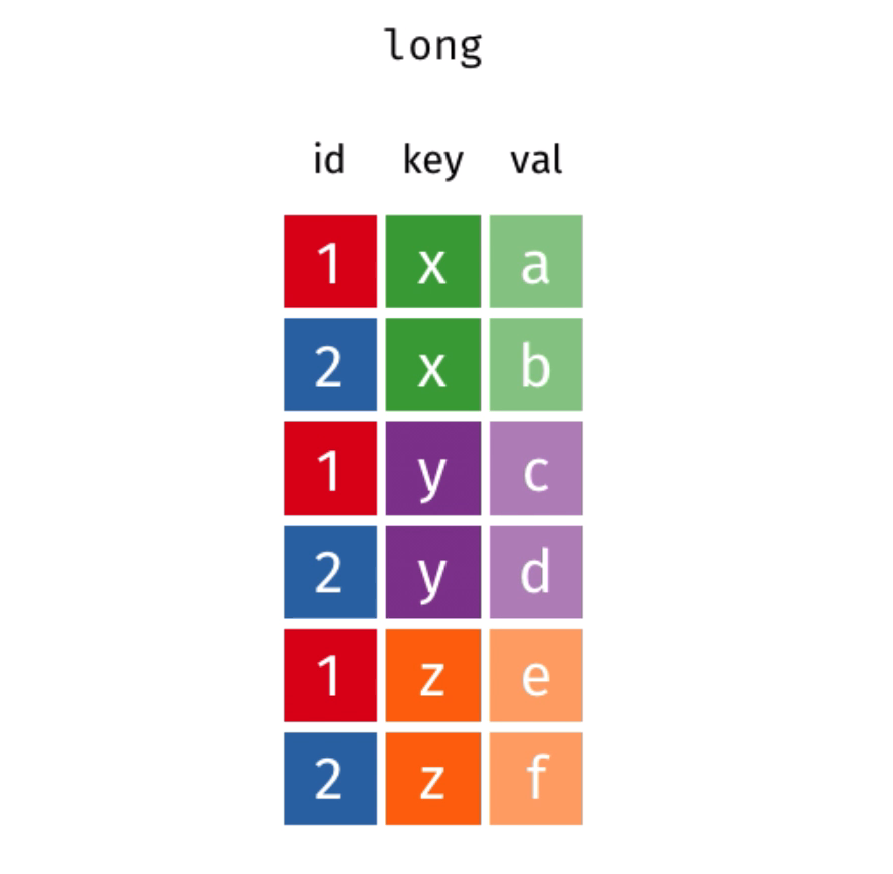
\includegraphics[scale = 0.25]{Masters-Thesis/img/tidyel2ws1.png} & 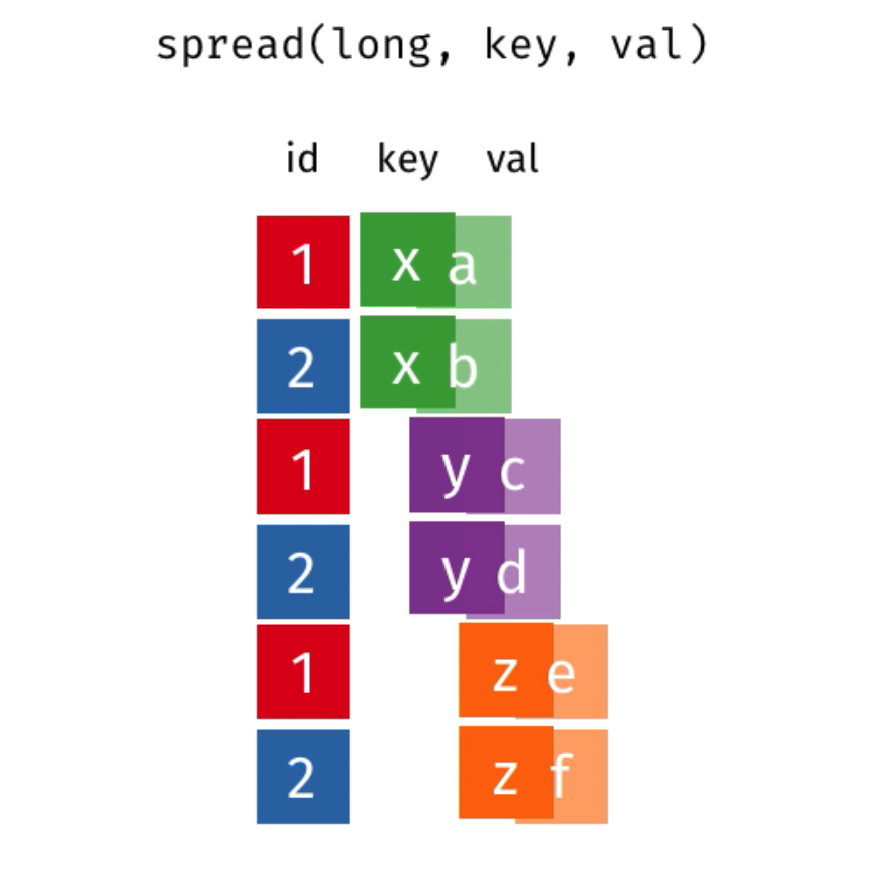
\includegraphics[scale = 0.25]{Masters-Thesis/img/tidyel2ws2.png} \\
    (a) Long to Wide step 1 & (b) Long to Wide step 2 \\[6pt]
     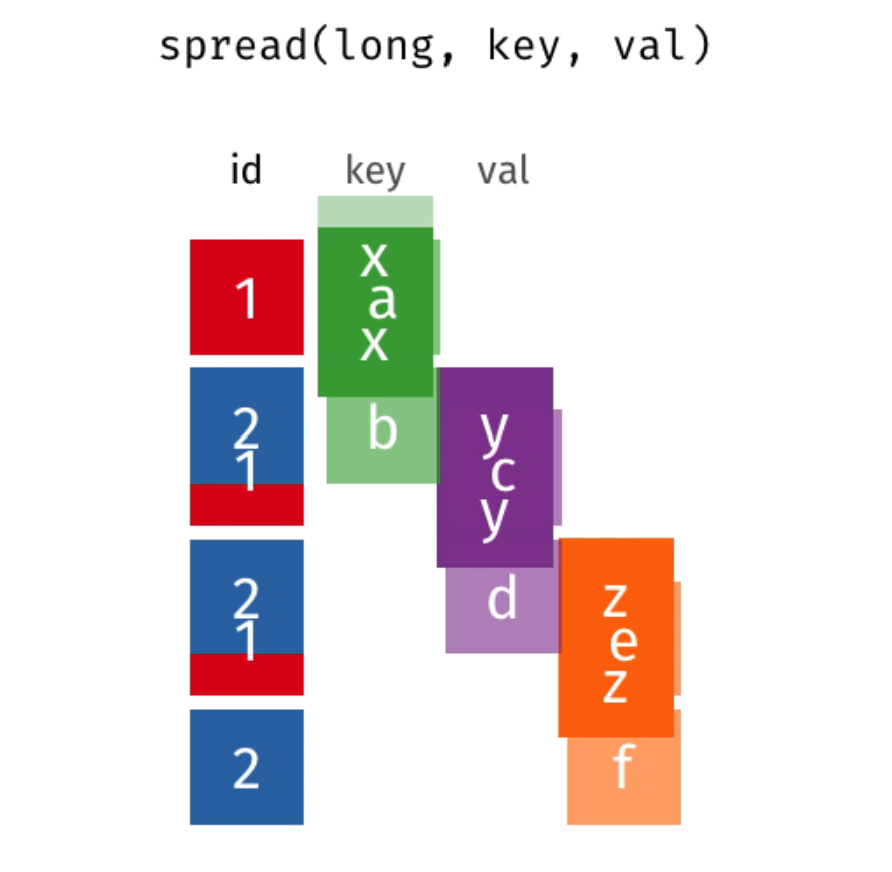
\includegraphics[scale = 0.25]{Masters-Thesis/img/tidyel2ws3.png} & 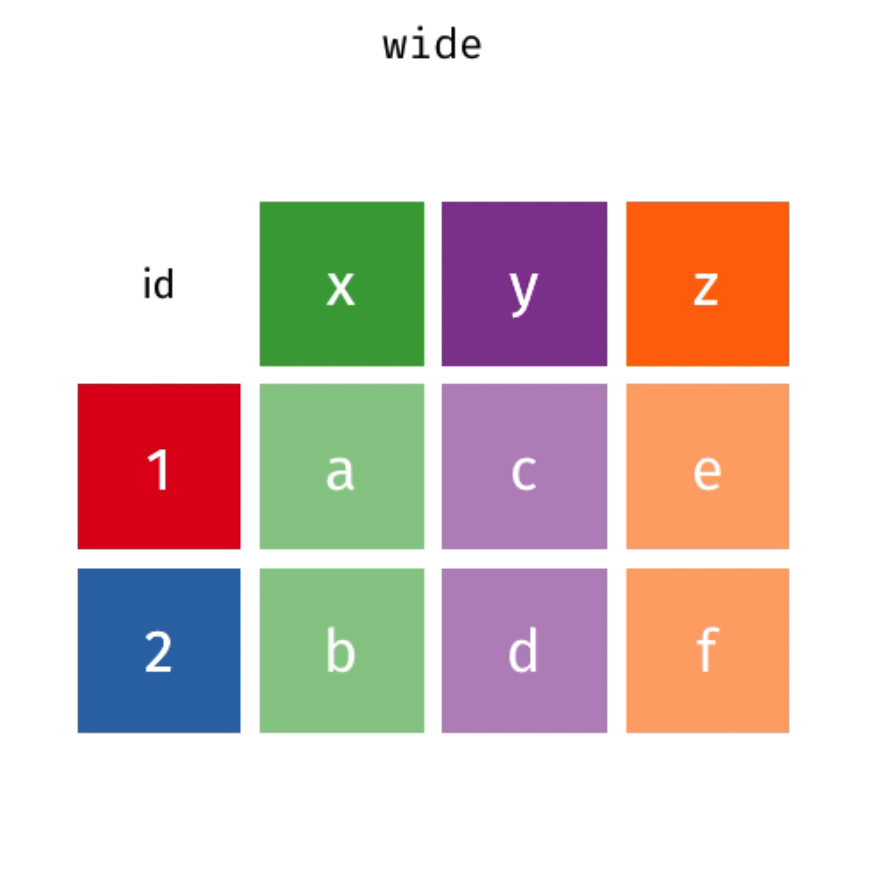
\includegraphics[scale = 0.25]{Masters-Thesis/img/tidyel2ws4.png} \\
    (c) Long to Wide step 3 & (d) Long to Wide step 4 \\[6pt]
    \end{tabular}
    \caption{Long to Wide in \textbf{tidyexplain}}
    \label{fig:tidyel2w}
\end{figure}
\newpage 
\begin{figure}[H]
    \begin{tabular}{cc}
     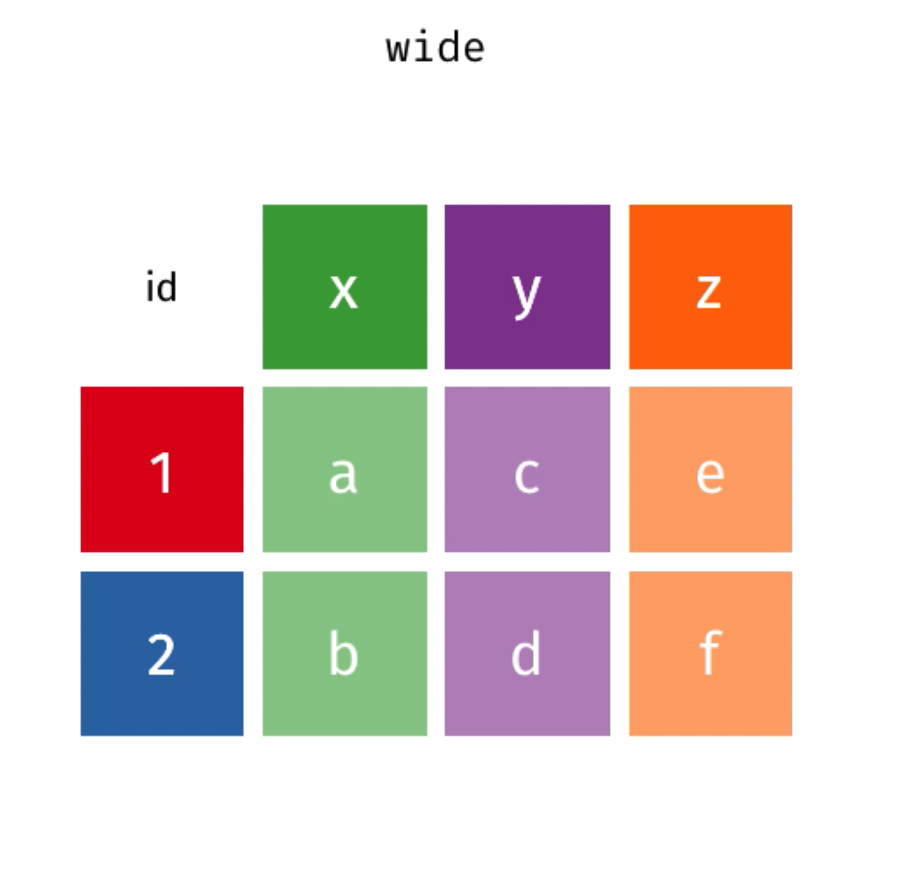
\includegraphics[scale = 0.25]{Masters-Thesis/img/tidyew2ls1.png} & 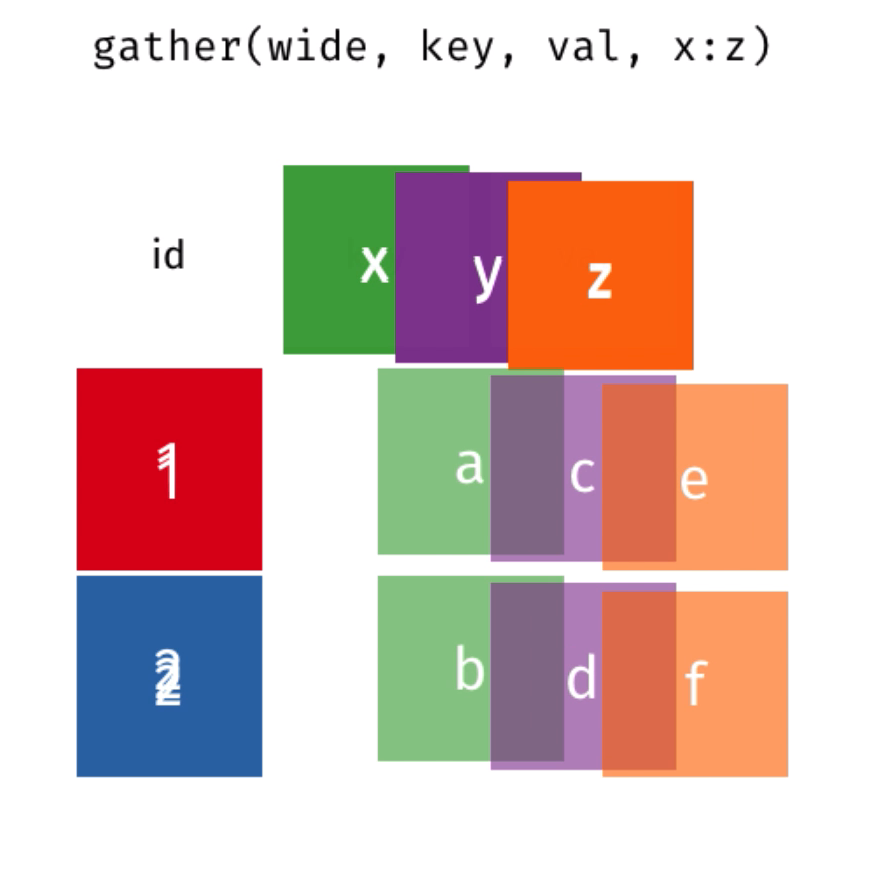
\includegraphics[scale = 0.25]{Masters-Thesis/img/tidyew2ls2.png} \\
    (a) Wide to Long step 1 & (b) Wide to Long step 2 \\[6pt]
     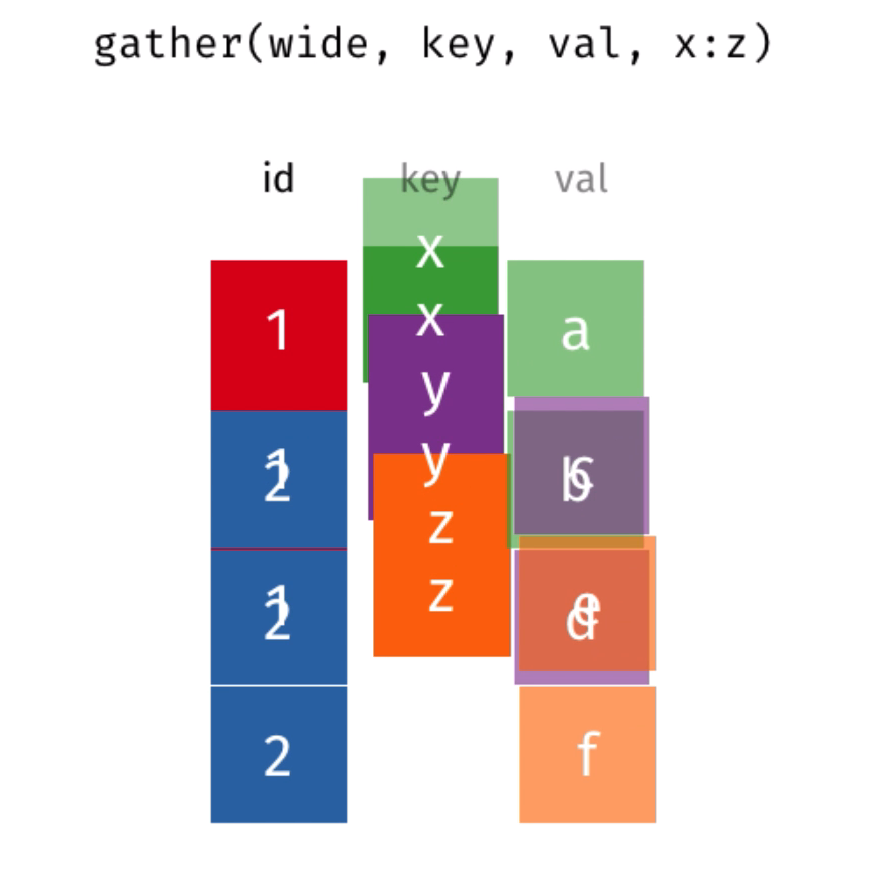
\includegraphics[scale = 0.25]{Masters-Thesis/img/tidyew2ls3.png} & 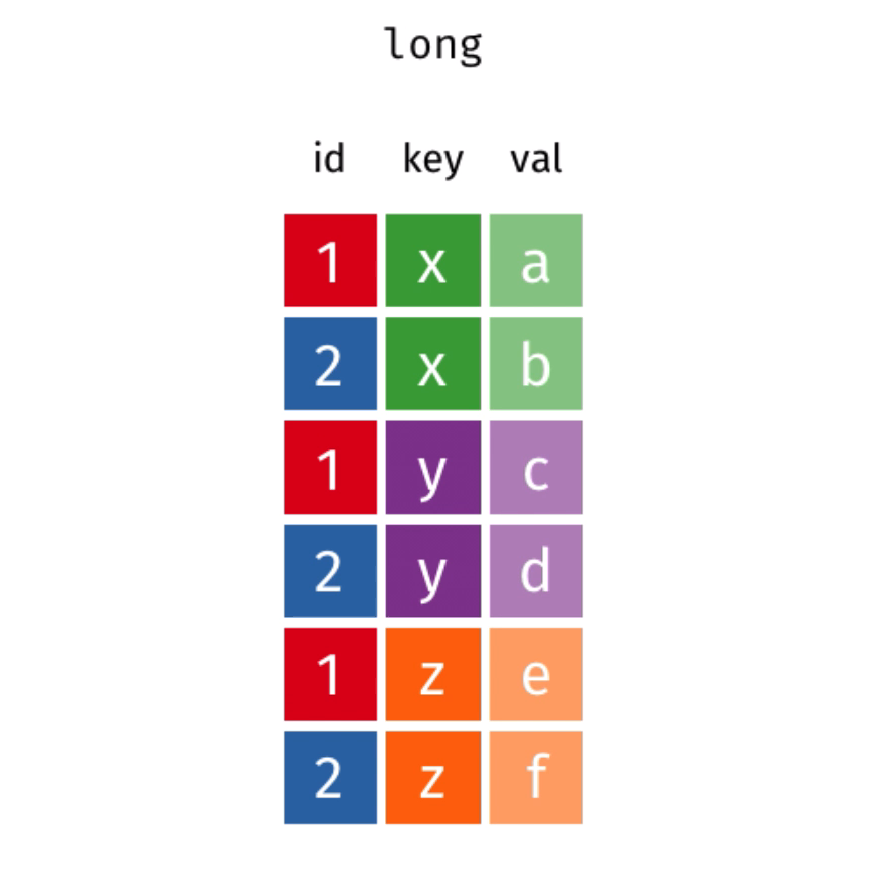
\includegraphics[scale = 0.25]{Masters-Thesis/img/tidyew2ls4.png} \\
    (c) Wide to Long step 3 & (d) Wide to Long step 4 \\[6pt]
    \end{tabular}
    \caption{Wide to Long in \textbf{tidyexplain}}
    \label{fig:tidyew2l}
\end{figure}


\newpage 
\section{Motivation}
The \textbf{tidyexplain} approach is a good start but there is more room for improvement. In general to make this more intuitive, we would like,
\begin{itemize}
    \item To allow users to input their own data to produce the animations.
    \item Displaying messages to show how the logic behind each step.
    \item Control of playback speed.
    \item Ability to save an animation for use in web pages and presentations. 
\end{itemize}

For the data joining module, we would like,
\begin{itemize}
    \item To allow for more advanced joins.
    \item Show why or how rows are joined together.
    \item Show how duplicated rows are handled. 
    \item Make the key column more stand out since it is the foundation of every join.
\end{itemize}

\newline 

For the data joining module, we would like,
\begin{itemize}
    % \item To animate more advanced reshaping transformations.
    % \item Show how or why certain elements are moved.
    \item To show how or why certain elements are moved.
    \item Show how elements within a table are related to each column or rows. 
    \item Convey the idea of key and value.
\end{itemize}